\documentclass[
    convert={density=300,outext=.png}
]{standalone}

\usepackage{graphicx}
\usepackage{tikz}
\usetikzlibrary{arrows,decorations.pathmorphing,positioning,fit}

\begin{document}
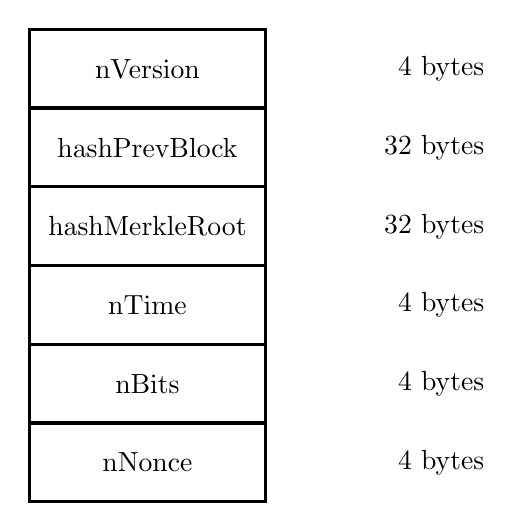
\begin{tikzpicture}
    [
        Field/.style={rectangle,minimum width=3cm,minimum height=1cm,draw,very thick,inner sep=1pt},
        TextBox/.style={minimum width=2cm, minimum height=1cm, text width=1.5cm, align=right}
    ]
    \node[Field] (nVersion) at (0,5)   {nVersion};
    \node[Field] (hashPrevBlock) at (0,4)  {hashPrevBlock};
    \node[Field] (hashMerkleRoot) at (0,3)  {hashMerkleRoot};
    \node[Field] (nTime) at (0,2)  {nTime};
    \node[Field] (nBits) at (0,1)  {nBits};
    \node[Field] (nNonce) at (0,0) {nNonce};

    \node[TextBox,right=of nVersion] (sizeof_nVersion) {4 bytes};
    \node[TextBox,right=of hashPrevBlock] (sizeof_hashPrevBlock) {32 bytes};
    \node[TextBox,right=of hashMerkleRoot] (sizeof_hashMerkleRoot) {32 bytes};
    \node[TextBox,right=of nTime] (sizeof_nTime) {4 bytes};
    \node[TextBox,right=of nBits] (sizeof_nBits) {4 bytes};
    \node[TextBox,right=of nNonce] (sizeof_nNone) {4 bytes};
\end{tikzpicture}

\end{document}